% ------------------------------------------------------------------------
% ------------------------------------------------------------------------
% ICMC: Modelo de Trabalho Acadêmico (tese de doutorado, dissertação de
% mestrado e trabalhos monográficos em geral) em conformidade com 
% ABNT NBR 14724:2011: Informação e documentação - Trabalhos acadêmicos -
% Apresentação
% ------------------------------------------------------------------------
% ------------------------------------------------------------------------

% Opções: 
%   Qualificação         = qualificacao 
%   Curso                = doutorado/mestrado
%   Situação do trabalho = pre-defesa/pos-defesa (exceto para qualificação)
\documentclass[qualificacao,mestrado]{packages/icmc}

% ---------------------------------------------------------------------------
% Pacotes Opcionais
% ---------------------------------------------------------------------------
\usepackage{rotating}           % Usado para rotacionar o texto
\usepackage[all,knot,arc,import,poly]{xy}   % Pacote para desenhos gráficos
% Este pacote pode conflitar com outros pacotes gráficos como o ``pictex''
% Então é necessário usar apenas um dos pacotes conflitantes
\newcommand{\VerbL}{0.52\textwidth}
\newcommand{\LatL}{0.42\textwidth}
% Comando simples para exibir comandos Latex no texto
\newcommand{\comando}[1]{\textbf{$\backslash$#1}}
% ---------------------------------------------------------------------------


% ---
% Informações de dados para CAPA e FOLHA DE ROSTO
% ---
% Tanto na capa quanto nas folhas de rosto apenas a primeira letra da primeira palavra (ou nomes próprios) devem estar em letra maiúscula, todas as demais devem ser em letra minúscula.

\tituloPT{Uma proposta de ontologia para o gerenciamento da fila de espera na atenção básica de saúde}

\tituloEN{An ontology proposal for the management of the queue in basic health care}
\autor[Guilherme, I. R.]{Igor Roberto Guilherme}
\genero{M} % Gênero do autor (M = Masculino / F = Feminino)
\orientador[Orientador]{Prof. Dr.}{Dilvan de Abreu Moreira}
%\coorientador{Prof. Dr.}{Fulano de Tal}
\curso{CCMC}
\data{03}{03}{2019} % Data do depósito
\idioma{PT} % Idioma principal do documento (PT = português / EN = inglês)
% ---


% ---
% RESUMOS
% ---

% Resumo em PORTUGUÊS
% conter no máximo 500 palavras
% conter no mínimo 1 e no máximo 5 palavras-chave
\textoresumo[brazil]{
O longo tempo de espera para o atendimento médico é um dos principais problemas do Sistema Único de Saúde (SUS). O tempo que um paciente é submetido a aguardar pelo atendimento, além de causar sofrimento, pode agravar a situação da enfermidade. A regulação destas filas é responsabilidade de cada município, que pode adotar enumeras formas de agendar um atendimento, não tendo a obrigatoriedade de expor os critérios de regulação. Em muitos casos são funcionários administrativos que realizam a gestão e ordenamento destas filas, sem ter um conhecimento aprofundado de cada caso para gerir de forma correta. Na literatura, há trabalhos que relatam casos de funcionários priorizando o atendimento de amigos e parentes. O computador por ser um item neutro, pode ajudar no gerenciamento destas filas, utilizando critérios definidos por especialistas. Para tal, é necessário que os dados estejam semanticamente representados, para a interpretação e gestão por parte das máquinas. A Web Semântica, através das ontologias permite a representação do conhecimento, possibilitando que as máquinas interpretem e auxiliem na gestão destas filas.
Desta forma, o presente trabalho propõe o uso das tecnologias da Web Semântica, mais precisamente ontologias OWL, para a representação dos indicadores para classificação de prioridades para o atendimento de uma especialidade médica. Como estudo de caso, uma ontologia OWL para o Hospital das Clínicas da Faculdade de Medicina de Marília (FAMEMA) e um protótipo que utilize esta ontologia e gerencie uma fila de retorno para uma especialidade médica será implementado. Almeja-se que o modelo proposto se mostre como uma boa alternativa ao modelo atual de gestão de filas, e que após uma validação por especialistas(médicos) o gerenciamento computacional seja mais justo se comparado a um gerenciamento anterior realizado no HC.
}{Fila de espera na saúde, Web Semântica, Sistema Único de Saúde, Ontologia}

\textoresumo[english]{The long wait time for medical care is one of the main problems of the Unified Health System (SUS). The time that a patient is submitted to waiting for the care, besides causing suffering, can aggravate the situation of the illness. The regulation of these queues is the responsibility of each municipality, which can adopt a number of ways to schedule a service, not having to state the regulatory criteria. In many cases they are administrative employees who manage and order these queues without having an in-depth knowledge of each case to manage correctly. In the literature, there are papers that report cases of employees prioritizing the care of friends and relatives. Because the computer is a neutral item, it can help manage these queues by using criteria defined by experts. For this, it is necessary that the data be semantically represented, for the interpretation and management by the machines. The Semantic Web, through ontologies allows the representation of knowledge, allowing the machines to interpret and assist in the management of these queues. In this way, the present work proposes the use of Semantic Web technologies, more precisely OWL ontologies, for the representation of the indicators for classification of priorities for attending a medical specialty. As a case study, an OWL ontology for the Hospital das Clínicas of Marília Medical School (FAMEMA) and a prototype that uses this ontology and manages a return queue for a medical specialty will be implemented. It is hoped that the proposed model will prove to be a good alternative to the current queuing management model, and that after a validation by specialists (physicians) the computational management will be more fair when compared to previous management performed in HC.
}{Waiting queue in health, Semantic Web,
Health Unic System, Ontology}
    
% ---
% Configurações de aparência do PDF final
% ---
\hypersetup{
	colorlinks=true     % false: boxed links; true: colored links
}
% --- 

% ----------------------------------------------------------
% ELEMENTOS PRÉ-TEXTUAIS
% ----------------------------------------------------------

% Inserir a ficha catalográfica
% \incluifichacatalografica{tex/ficha-catalografica.pdf}

% DEDICATÓRIA / AGRADECIMENTO / EPÍGRAFE
%\textodedicatoria*{tex/pre-textual/dedicatoria}
%\textoagradecimentos*{tex/pre-textual/agradecimentos}
%\textoepigrafe*{tex/pre-textual/epigrafe}

% Inclui a lista de figuras
\incluilistadefiguras

% Inclui a lista de tabelas
\incluilistadetabelas

% Inclui a lista de quadros
% \incluilistadequadros

% Inclui a lista de algoritmos
%\incluilistadealgoritmos

% Inclui a lista de códigos
%\incluilistadecodigos

% Inclui a lista de siglas e abreviaturas
\incluilistadesiglas

% Inclui a lista de símbolos
%\incluilistadesimbolos

% ----
% Início do documento
% ----
\begin{document}
% ----------------------------------------------------------
% ELEMENTOS TEXTUAIS
% ----------------------------------------------------------
\textual

\chapter{Introdução}
\label{chapter:introducao}
A fila de espera faz parte do nosso cotidiano, enfrentamos filas para diversos objetivos, seja no supermercado, em Bancos e até mesmo para um atendimento médico. No caso dos serviços de saúde, a longa espera pode propiciar o sofrimento do paciente, reduzir as possibilidades de cura, permitir o agravamento das enfermidades ou a extensão das sequelas e até determinar risco de morte \cite{Gazzinelli2014}. 

No Sistema Único de Saúde(SUS), marcar consulta com especialista é o maior problema para os brasileiros \cite{CFM2018}. Não há um modelo claro de regulação do SUS, ficando a cargo de cada município gerir as filas de espera para os atendimentos especializados. A gestão destas filas ocorre de maneira manual, em muitos casos por funcionários das unidades de saúde que não obtém de um conhecimento  amplo para identificar e comparar casos de cada enfermidade. Neste cenário, os funcionários adotam um agendamento das consultas, predominantemente, pela ordem de chegada das fichas de encaminhamento na recepção, exceto quando o médico sinaliza a urgência no atendimento do caso, como relatado no trabalho de \cite{SOUZA2014}.

Apesar de fazer parte do dia-a-dia dos médicos que trabalham em serviço público, o problema da fila de espera é muito pouco abordado pela comunidade médica e científica, talvez por parecer tratar-se de uma discussão que não pertence aos meios acadêmicos e sim às instâncias governamentais. Todavia é preciso salientar que o acesso equitativo, justo e universal aos serviços de saúde deve ser uma preocupação constante não só do governo como de todos os profissionais envolvidos no atendimento à rede pública. Muito pode ser feito em nível local a respeito das filas de espera. \cite{KRISHNAMURTI2005}

O tempo de espera é um indicador da qualidade dos serviços, por estar relacionado à capacidade de resposta do sistema às necessidades de atenção à saúde da população \cite{Gazzinelli2014}. 

A tecnologia é muito importante para a gestão de saúde,
ultrapassando o processamento-padrão de dados para funções administrativas comuns em todas as organizações, tais como recursos humanos, folhas de pagamento, sistemas de contabilidade, entre outros, e agora desempenha um papel fundamental tanto no cuidado ao paciente, na interpretação do eletrocardiograma, como em escalas de trabalho, prescrição, relatório de resultados e sistemas de prevenção \cite{PINOCHET2014}. O computador pode auxiliar no processamento de informações de saúde, para \cite{MATTOS1978}, as tarefas realizadas pelo computador, desde que corretamente programado, são praticamente isentas de erro, o que não ocorre no caso do processamento manual (realizado por pessoas). O trabalho ainda relata que o principal motivo dessa perfeição é que a máquina não é sensível aos fatores que reduzem a qualidade do trabalho humano, quais sejam:

  \begin{enumerate}
    	\item a fadiga - que faz com que o número de erros cometidos involuntariamente aumente ao fim do turno de trabalho;
        \item Dos problemas pessoais - uma preocupação com a família, por exemplo, perturba bastante o bom desempenho do funcionário;
        \item o desajuste com a empresa - um empregado mal pago, ou ameaçado de ser despedido, "vinga-se" da empresa sabotando o sistema de informações do qual participa;
        \item interesses pessoais - o funcionário procura adulterar o sistema em beneficio próprio. Tal é o caso, por exemplo, da emissão de uma ordem de serviço para a instalação de um telefone em uma loja comercial, passando na frente de centenas de outros clientes, por um empregado" que recebe uma propina do proprietário dessa loja;
        \item desorganização e falta de planejamento - a incapacidade de um chefe pode desorientar seus subordinados, reduzindo a qualidade de seu serviço.
    \end{enumerate}
    
O trabalho apresenta os itens com uma visão mais empresarial, porém, é possível ter um entendimento com um olhar sobre os funcionários gestores das filas de espera para o encaminhamento especializado. O item 4 por exemplo, é perfeitamente comparável a de funcionários que priorizam o atendimento de amigos e parentes na gestão destas filas, conforme citado no trabalho de \cite{KRISHNAMURTI2005}

A Web Semântica é uma destas tecnologias que podem auxiliar processos na área da saúde. Atrvés da OWL - Ontology Web Language, criada pela World Wide Web Consortium (W3C), é possível tornar as informações, antes apenas compreensível por humanos, em informações passíveis de interpretação por computadores. O gerenciamento das filas de espera por parte dos computadores, pode contribuir para se alcançar filas isentas de fatores humanos (descritos na lista anterior), ainda possibilitar a redução do tempo de espera para os pacientes que precisam de um atendimento imediato de acordo com suas características físicas e sociais. 

Como uma instância destas lacunas é possível citar o caso do Hospital das Clínicas da Faculdade de Medicina de Marília(FAMEMA), onde o problema da fila de espera ocorre em casos de retorno de um paciente a uma especialidade, cuja fila é denominada como "Demanda". Na Demanda, é utilizado o método tradicional de fila(First In, First Out - FIFO), gerando "filas sem fim", nas quais os pacientes chegam a esperar mais de oito anos por um atendimento. No gerenciamento da Demanda, ainda não é levado em consideração o quadro clínico do paciente, tais como o diagnóstico, gravidade, idade e a capacidade de um paciente se recuperar de uma enfermidade no caso da urgência no seu retorno. A demanda é distribuída por profissional e não por especialidade, necessitando que em casos de desligamento de algum profissional, a distribuição manual da fila para outros médicos.

Um efeito colateral do gap entre a entrada do paciente na Demanda e o seu efetivo atendimento é o absenteísmo. Por vários motivos: o problema inicial para o qual o paciente procurou atendimento não existe mais, foi atendido por outro estabelecimento/profissional de saúde, o paciente não foi localizado, o paciente veio a óbito, entre outros. 



\section{Objetivos}
    O objetivo deste trabalho é analisar as filas de espera do Sistema Único de Saúde (SUS), mais precisamente no encaminhamento do atendimento básico para o atendimento especializado, e propor um modelo computacional para o gerenciamento dessas filas, com o intuito de torná-las mais coerentes com a prioridade de atendimento definida por especialistas (médicos), sem a necessidade da alocação de um profissional dedicado à essa função. 
    
    Ainda pretende-se obter filas mais justas,  minimizando a possibilidade de indivíduos serem atendidos prioritariamente por terem acesso aos gestores dessas filas, como citado no trabalho de \citeonline{KRISHNAMURTI2005}. Objetiva-se que os critérios de ordenamento da fila sejam mais transparentes, e que o posicionamento de cada paciente seja feito com isenção, levando em consideração apenas a situação física e social de cada um.

\subsection{Objetivos específicos}

	Para alcançar os objetivos apresentados na seção anterior, foram definidos os objetivos específicos:
    
    \begin{itemize}
    	\item Criação de uma ontologia de domínio no formato OWL que represente indicadores para classificação de prioridades para o atendimento de uma especialidade médica.
        \item Desenvolvimento de um protótipo que utilize a ontologia e, de acordo com critérios médicos, gerencie uma fila de espera.
        \item Acompanhamento da avaliação dos médicos do Hospital das Clínicas da Faculdade de Medicina de Marília do protótipo com o intuito de verificar como o gerenciamento computacional se  sobressai se comparado ao gerenciamento atual do HC.
    \end{itemize}


\section{Organização do Trabalho}

	A presente dissertação está organizada da seguinte forma:
	
    \begin{itemize}
    	\item Capítulo 2: Apresenta os conceitos relevantes que estão relacionados com o este trabalho;
        \item Capítulo 3: Expõe as características dos trabalhos relacionados;
        \item Capítulo 4: Descreve a proposta da pesquisa, a metodologia utilizada e o cronograma detalhado de cada atividade.
    \end{itemize}

\chapter{Referencial Teórico}
\label{chapter:referencial-teorico}
Neste capítulo são apresentados em cada subseção conceitos importantes para a construção e melhor compreensão deste trabalho.

\section{Fila de espera no Sistema Único de Saúde}
    O Sistema Único de Saúde (SUS) é um dos maiores sistemas públicos de saúde do mundo, sendo o único a
    garantir assistência integral e completamente gratuita para a totalidade da população \citeonline{SOUZA2002}. Diferentemente de outros países, no Brasil, mesmo quem opta por um plano de saúde privado tem o direito de ser atendido em qualquer unidade do Sistema Único de Saúde.
   
   \subsection{Financiamento do SUS}
   
     O financiamento do SUS é uma responsabilidade comum entre o governo nacional, estadual e municipal que realizam a destinação de porcentagens diferentes de seu orçamento para o SUS, dividia da seguinte forma \citeonline{CONASS}:
    \begin{itemize}
        \item União: A Emenda Constitucional n. 86 de 17 de março de 2015 definiu que a partir de 2016 a União aplicará, anualmente, em ações e serviços públicos de saúde, o montante correspondente ao valor da Receita Corrente Líquida (RCL) do respectivo exercício financeiro, não podendo ser inferior a 15\%, mas que será cumprido progressivamente
        \item  Estados e Distrito Federal: No mínimo 12\% da arrecadação dos impostos são destinadas a ações e serviços públicos de saúde, sendo deduzidas as parcelas que forem transferidas aos municípios;
        \item Municípios e o Distrito Federal: Anualmente aplicam em ações e serviços públicos de saúde, no mínimo, 15\% da arrecadação dos impostos.
    \end{itemize} 

   
   	\subsection{Funcionamento do SUS}
   	
    O Governo Federal tem o dever de fiscalizar e elaborar mecanismos de apoio para que  estados e municípios possam oferecer serviços de saúde.

   É na instância municipal que o paciente dá a entrada no sistema, por meio da UBS (Unidade Básica de Saúde) ou pela equipe da Unidade Saúde da Família (USF) que são profissionais que acompanham um número de famílias em uma determinada área geográfica. Na UBS é realizado o atendimento com hora marcada e deve sempre haver médicos de três especialidades: clínico geral, pediatra e ginecologista. Nestas unidades é oferecido um primeiro atendimento, afim de realizar uma triagem e quando necessário solicitar o encaminhamento para as demais especialidades \citeonline{CONTE2017}.
   
   Na imagem XX abaixo, é apresentado o fluxo pelo qual o paciente é submetido dentro do SUS desde o primeiro contato até um atendimento especializado ou internação:
    
     \begin{figure}[htbp]
        	\centering
            \caption{Funcionamento SUS}
            \label{fig:images/fluxograma-trajetoria-usf-pe}
            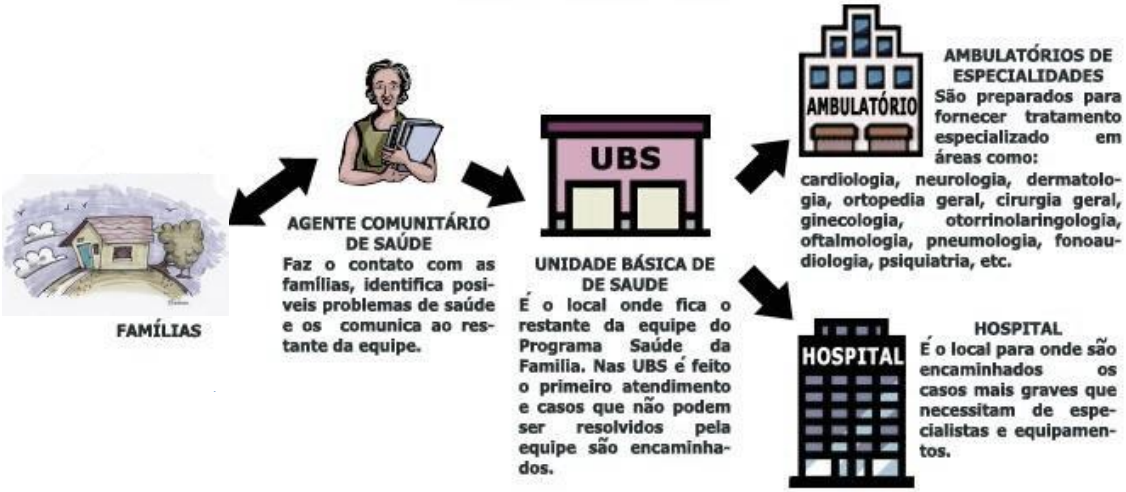
\includegraphics[width=0.9\linewidth]{images/funcionamento-sus.png}
            \fdireta{SECRETARIAMG}
        \end{figure}
    
    Ainda na UBS, caso o paciente necessite de um atendimento emergencial, a UPA (Unidade de Pronto Atendimento) é quem o recebe. As UPAs são unidades de complexidade intermediária entre  as UBSs e a emergência dos hospitais, portanto, servem para "desafogar" as filas dos hospitais. Segundo o Ministério da Saúde, 97\% dos casos que chegam as UPAs são solucionados \citeonline{BRASIL2012}. Os pacientes que procuram as UPAs são avaliados de acordo com a classificação de risco, ou seja, os casos mais graves terão prioridade.
    
     \subsection{Filas de espera}
    
    O caminho que um paciente percorre até o efetivo atendimento pode ser longo e muitas vezes acaba precisando retornar no início do fluxo de atendimento. O trabalho de \citeonline{SOUZA2014}, avaliou as condições de acesso integral dos usuários a partir do caminho percorrido desde a atenção básica até a especializada na rede assistencial de Recife - PE. O fluxograma do caminho percorrido pelos pacientes é exibido na figura XX:
    
     \begin{figure}[htbp]
        	\centering
            \caption{Fluxograma Descritor do acesso do usuário da atenção primária à atenção especializada.}
            \label{fig:images/fluxograma-trajetoria-usf-pe}
            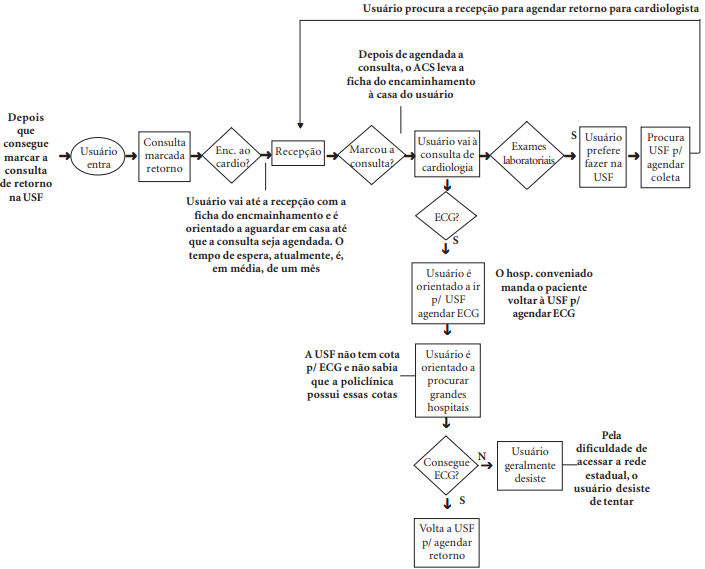
\includegraphics[width=0.8\linewidth]{images/fluxograma-trajetoria-usf-pe}
            \fdireta{SOUZA2014}
        \end{figure}
        
    Quando um médico de família encaminha um usuário ao especialista, este procura a recepção da USF para entregar a sua ficha de encaminhamento ao profissional responsável pela marcação das consultas que por sua vez faz o contato telefônico com a Central de Regulação do Recife para o agendamento.
    A demora no agendamento das consultas especializadas é uma das barreiras de acesso para o atendimento integral da população. No estudo, ainda é citado que a inexistência de critérios definidos para a escolha do serviço de referência no qual os usuários serão agendados é outro aspecto desordenador do acesso, essa definição cabe ao pessoal administrativo, ou os ‘marcadores das consultas’. Outro aspecto que chama a atenção, como
    elemento desordenador, é o fato de o agendamento das consultas ser realizado, predominantemente, pela ordem de chegada das fichas de encaminhamento na recepção. Com exceção dos casos em que o próprio médico sinaliza a ‘urgência’ ou ‘prioridade’ dos pacientes, é o responsável pela marcação das consultas que tenta priorizar
    quem deverá ter acesso e agendamento prioritário. Esse aspecto demonstra que a análise de risco clínico não se coloca como atividade consolidada no processo de trabalho das equipes de saúde da família \citeonline{SOUZA2014}.
    
    Um outro problema abordado na literatura quando se trata de atendimento especializado, é a questão do absenteísmo. No trabalho de \cite{URSULA2018} é realizada uma análise do impacto da fila da espera no absenteísmo de exames e consultas. O estudo revela que as maiores
    probabilidades de ocorrência de absenteísmo são obtidas de modo geral em
    procedimentos que ultrapassam os 60 dias de espera. O trabalho concretiza que a redução do tempo de espera para menos de 60 dias possibilitou a diminuição significativa do absenteísmo, o que repercute na diminuição do agravamento de doenças e nos custos ao sistema de saúde. 
    
    A fila de espera não é um entrave apenas no SUS, é um problema em cerca da metade dos países da OECD \cite{SICILIANI2004}. Recursos financeiros escaços, quantidade de vagas, gestão e estrutura são também presentes em outros países, como o Sistema Nacional de Saúde espanhol (SNS). No trabalho de Conill (2011), para o enfrentamento destas barreiras no acesso ao sistema de saúde, foram realizadas iniciativas que a proporcionassem a continuidade assistencial. Foi adotada a medida de circuitos preferenciais. Essa estratégia serve para encaminhar da atenção primária com preferência os usuários com suspeitas de alguma etiologia específica. Uma parceria entre o Fórum Espanhol de Pacientes em conjunto com a Universidade de Harvard (EUA), desenvolveu uma pesquisa com 3.010 cidadãos, para avaliar a confiança dos espanhóis no sistema nacional de saúde. Entre outros aspectos, este trabalho revelou que, sem distinção de classe social, área geográfica ou densidade demográfica, as listas de espera são o principal problema dos serviços de saúde espanhóis para 78\% dos entrevistados. \citeonline{LOPEZ2007} 
    Vale salientar que as filas de espera do atendimento básico para o especializado, não são as únicas onde o paciente encontra problemas, filas como de urgências e cirurgias também são dificuldades reais no SUS. O trabalho de \citeonline{KRISHNAMURTI2005}, trás uma abordagem das filas de espera para cirurgias otorrinolaringológicas no SUS. O trabalho descreve que o maior afunilamento acontece na obtenção da consulta no ambulatório de otorrinolaringologia, ou seja no atendimento especializado (seta nº 3, na figura XX).
    
    \begin{figure}[htbp]
        	\centering
            \caption{As setas tracejadas representam os pontos críticos no processo de obtenção do tratamento.}
            \label{fig:images/fluxo-fila-cirurgia-otorrino}
            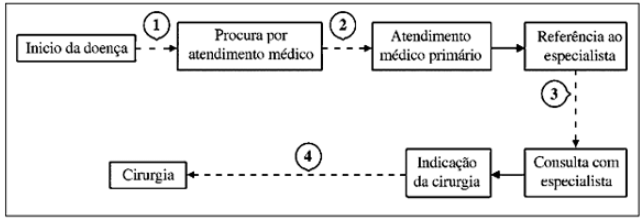
\includegraphics[width=0.9\linewidth]{images/fluxo-fila-cirurgia-otorrino.png}
            \fdireta{KRISHNAMURTI2005}
        \end{figure}
        
    O trabalho ainda discute um tema importante, ao questionar se os indivíduos destas filas de espera realmente passaram por vias regulares e justas para o atendimento. Muitos que tem a possibilidade, procuram outras formas de se obter a consulta, surgem então os pedidos de "consulta extras". São os chamados "PAFs" ou "PAFUNCIOs" tão conhecidos do médico que trabalha em serviço público: "Parente ou Amigo de Funcionário".

    No artigo, o autor relata que ocorre uma pressão não só diretamente sobre os médicos, mas também sobre enfermeiros, auxiliares de enfermagem e demais funcionários. Os funcionários responsáveis pela marcação das consultas também são pressionados, de modo que é preciso atentar para o fato de que mesmo o paciente que parece ter tido a sua consulta marcada por vias regulares pode ter sido beneficiado nessa marcação. Mais grave, já há casos (crimes, melhor dizendo) de pessoas e funcionários que vendem estas consultas ou mesmo um lugar na fila da triagem do hospital. O médico, sem saber, passa a ser o instrumento de um lucrativo negócio: o do agenciamento da medicina pública \citeonline{KRISHNAMURTI2005}.
    Estes pacientes, independente da gravidade de suas queixas e do seu direito inquestionável ao atendimento, estão na realidade "furando" uma fila virtual de espera. Pode-se chegar a extremos em que o número de pessoas "furando" a fila é tal a ponto de criar uma fila paralela, com fluxo contínuo, enquanto a fila principal e legítima permanece quase parada. Concluindo, o trabalho ainda deixa claro que é necessário o enfrentamento da questão, e que os pacientes devem ser informados sobre sua condição, de preferência por escrito, da indicação cirúrgica, da existência da fila, dos critérios de prioridade nesta fila, da quantidade de pessoas à sua frente e de uma estimativa do tempo até sua cirurgia, deixando-se claro tratar-se apenas de uma estimativa.
    
    --TOPICO DESENVOLVIMENTO
    
    SUBTOPICO DE DESENVOLVIMENTO, Critérios para priorização doa tendimento:
    
    Entende-se por prioridade no atendimento cirúrgico a própria ordem em que estes pacientes serão atendidos, isto é, submetidos à cirurgia. Até então consideramos o tempo de espera na fila como o principal critério de prioridade. Entretanto, este não é obviamente o único critério que deve ser considerado. Pacientes que necessitam de cirurgias de emergência (uma mastoidite aguda ou uma sinusite com complicação intra-orbitária) são exemplos extremos em que a prioridade independe do tempo de espera.

Da mesma forma, mesmo em cirurgias eletivas, a prioridade na realização da cirurgia deve também levar em conta a gravidade e urgência de cada caso. Pacientes com casos mais graves devem ser operados antes daqueles com casos menos graves, independente do tempo de acompanhamento no serviço. É preciso, todavia, que estes critérios de prioridade sejam claros e bem estabelecidos para um bom funcionamento do serviço.

Por gravidade, entenda-se o grau de sofrimento, limitações ou risco de vida que a doença impõe ao paciente. O conceito de urgência leva em conta a gravidade aliada aos possíveis benefícios da cirurgia em relação à história natural da doença, além de fatores sociais e filosóficos7. Um paciente com câncer de laringe em estado inicial, por exemplo, não é um caso grave no momento, uma vez que só apresenta disfonia leve, mas é um caso urgente pois a cirurgia tem grande impacto na evolução da doença. Por outro lado, um paciente em estado terminal é sem dúvida um paciente grave, mas não urgente pois a cirurgia tem menor impacto na história natural de sua doença. É com base nestes conceitos que cada serviço deve estabelecer seus critérios de prioridade para cada cirurgia.

Em linhas gerais, alguns critérios devem ser destacados:

1. História de complicações

a. Complicações sistêmicas. 
b. Complicações em órgãos e estruturas adjacentes. 
c. Complicações locais.

1. Pacientes com comorbidades graves. 
2. Pacientes com sinais clínicos ou radiológicos de doença avançada. 
3. Menores de idade e idosos. 
4. Fatores sócio-econômicos.

O histórico de complicações infecciosas ou de outra natureza é talvez o critério de prioridade mais importante, pois representa um risco aumentado de óbito. As complicações devem ser estratificadas em seus graus de severidade e possibilidade de recorrência. Como regra geral, as complicações infecciosas intra-cranianas (meningite, abscesso intra-craniano, empiema) são consideradas mais graves, pelo risco de vida e alta taxa de recorrência. Em seguida vêm as complicações em órgãos adjacentes (como as orbitárias na polipose nasal) e restritas ao órgão alvo da doença (como a paralisia facial no colesteatoma).

Os pacientes com comorbidades graves são outro grupo prioritário. Entenda-se por comorbidade outras afecções sistêmicas com ou sem relação com a doença otorrinolaringológica e que a revestem de maior gravidade ou possibilidade de complicação pela interação mútua das duas condições. Exemplos clássicos são a associação entre polipose e asma ou entre hipertrofia adenoamigdaliana e síndrome de apnéia obstrutiva do sono. Entretanto, outras afecções sistêmicas, mesmo sem relação direta com a doença otorrinolaringológica, devem ser levadas em conta, tais como insuficiência renal, transplantados (ou candidatos a transplante), pacientes com SIDA, diabéticos graves, etc.

Pacientes com sinais clínicos ou radiológicos de doença avançada que sugiram a possibilidade aumentada de evolução para complicações também devem ser priorizados. Colesteatomas com erosão avançada do tegmen timpani encaixam-se neste grupo.

Pelo estatuto da criança e do adolescente8 e pelo estatuto do idoso9, ambos já em vigor em nosso país, estes grupos etários devem sempre ser priorizados no atendimento em qualquer hospital público e na implantação de qualquer política de saúde. Portanto, também devem ser considerados casos prioritários.

Já os fatores sócio-econômicos são sem dúvida importantes, mas a sua consideração no estabelecimento dos critérios de prioridade é bastante controversa. Alguns serviços, por exemplo, priorizam a cirurgia de pacientes que moram em municípios distantes ou mesmo em outros estados, por entenderem que o acompanhamento prolongado em hospital tão distante de suas residências causa transtorno e sofrimento maiores. Outros podem considerar relevantes questões mais sutis, como o impacto da doença na vida profissional do paciente, ou o caso de pacientes que cuidam de parentes doentes e que portanto não têm tempo para cuidar de sua própria saúde, etc. As possibilidades são infinitas. Por isso é necessário que haja abertura para ampla discussão dos critérios a serem estabelecidos e também para casos particulares. O uso do livre entendimento e do bom senso da equipe cirúrgica não pode ser negligenciado, desde que se aplique sempre os mesmos critérios para todos os casos.
(http://www.scielo.br/scielo.php?script=sci_arttext&pid=S0034-72992005000300001)
    

--citar conil e ver se el falar isso mesmo
Além desses casos, no aspecto de organização, a fila de espera pode adotar
na prática outros recursos de ordenamento. Sarmento Júnior, Tomita e Kos. (2014)
abordam o recurso da fila do “esperar para ver” (“wait and see list”), como uma boa
alternativa para gerenciar os casos etiológicos que podem ser “tratados” durante o
tempo de espera. Esses casos são monitorados e transferidos de fila. Um exemplo
apontado pelos autores são os casos de cirurgias oftalmológicas. Cria-se uma fila
para os casos que a indicação para cirurgia ainda não é exata, fazendo então o
acompanhamento desses pacientes, para um futuro encaminhamento para a fila
conforme o retrocesso ou avanço de uma patologia.
Contudo, a literatura apresentou os dados estatísticos das taxas crescentes
do impacto da fila de espera e a importância de implantar ferramentas que auxiliem
no processo de otimização dos serviços de saúde, nesse caso, voltado para os
fatores que interferem na fila de espera e nas perdas causadas pelo absenteísmo.
Ou seja, adotar alternativas para diminuir esse problema no sistema de saúde e
buscar atender as necessidades do município com relação à oferta de serviços
especializados (ALBIERI, 2015).
Em nível nacional faz-se necessário incremento na estratégia de regulação,
que fomenta a efetivação do ordenamento do de acesso aos serviços de saúde
    
    -colocar na instrocução o conteudo abaixo
    
    Como o número de pacientes que necessitam de um atendimento especializado é maior que a quantidade de vagas oferecidas, uma fila de espera é criada. A fila de espera é uma lista de pacientes que necessitam de um mesmo tratamento ou serviço médico cuja demanda é maior que a oferta.\citeonline{KRISHNAMURTI2005} As
    especialidades médicas e os serviços de exames possuem uma capacidade limitada de atendimentos, isto é, um número finito de vagas.
    
    Longos tempos de espera têm se constituído em um problema comum em diferentes sistemas públicos de saúde. Além de um importante determinante da satisfação dos profissionais e usuários, o tempo de espera é um indicador da qualidade dos serviços, por estar relacionado à capacidade de resposta do sistema às necessidades de atenção à saúde da população. \citeonline{Gazzinelli2014} No Brasil, o longo tempo de espera para consultas especializadas está entre as principais barreiras ao acesso a cuidados integrais à saúde no Sistema Único de Saúde (SUS).
    
    Não há controle das listas de espera ou uma estratégia padrão para organizá-las. Ficando a critério das instituições a escolha da forma que sistematizará, se por especialidade, prestador ou por data, gerando então diversas filas e informações que dificultam inclusive o monitoramento e gerenciamento das mesmas \citeonline{URSULA2018}.
    
    Como cada município pode fazer a gestão da fila, nem sempre é um especialista que elabora a fila de espera, podendo ainda não utilizar critérios corretos para a ordem de atendimento. Algumas possíveis soluções para o problema da fila de espera merecem discussão. Medidas que aumentem a oferta de serviços especializados estão, frequentemente, entre as principais estratégias para a redução do tempo de espera. Mas entende-se que simplesmente aumentar a oferta de consultas, visando reduzir a lista de espera, apenas encorajaria o número de encaminhamentos. A solução passa também, provavelmente, por melhor comunicação entre o médico clínico geral, ou médico de comunidades, e o especialista. Para isso, é necessária estruturação adequada e consistente dos serviços de atenção primária, com melhorias nos sistemas de agendamento e de encaminhamento.\citeonline{Gazzinelli2014}
    
  

\section{Web Semântica e Ontologia}

	Apesar de ser criada para possibilitar o acesso, intercâmbio e recuperação de informação de forma simples e rápida, o crescimento caótico e exponencial da \textit{Web} fez com que ela se tornasse um enorme repositório de documentos, dificultando o processo de recuperação dos mesmos \cite{Suarez2017}. Ainda hoje não existe nenhuma estratégia abrangente e satisfatória o suficiente para organizar documentos por meio de motores de busca que seja coerente com uma estrutura linguística \cite{Ci.Inf.1077}. Um outro exemplo de deficiência da \textit{Web} atual pode ser identificado em buscas feitas em sistemas de recuperação de informação, que usam palavras-chave nas buscas, considerando apenas o grau de similaridade e nível de ocorrência de certas palavras no documento, ou seja, a semântica da busca é desconsiderada \cite{Ci.Inf.1077}.
    
    Apresentada por \citeonline{10.2307/26059207}, a Web Semântica surge como uma proposta de estruturar os dados e informações disponíveis na \textit{Web}, para que agreguem significado e passem a ser computáveis por máquinas. A Web Semântica é definida por um conjunto de padrões definidos pela organização chamada \sigla{W3C}{World Wide Web Consortium}. Na sua proposta original, ela é definida como um extensão da \textit{Web} atual que tem como objetivo criar uma \textit{Web} universal dos conhecimentos da humanidade.
    
    Partindo dessa visão conceitual, \citeonline{10.2307/26059207} propuseram uma arquitetura de representação do conhecimento por camadas, conhecida pelos nomes de \textit{Semantic Web Stack}, \textit{Semantic Web Cake} e \textit{Semantic Web Layer Cake}, ilustrada na \autoref{fig:semanticcake}.
    
    \begin{figure}[htb]
    	\centering
        \caption{Arquitetura em camadas da Web Semântica.}
    	\label{fig:semanticcake}
        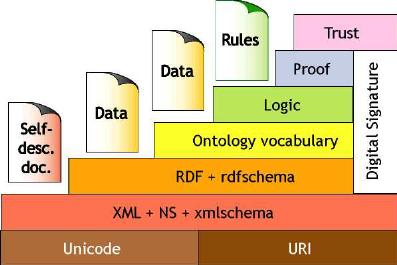
\includegraphics[width=0.7\linewidth]{images/semantic-web-cake}
        \fdireta{MIKA2005}
    \end{figure}
    
    A partir das bases \textit{Unicode} e \textit{URI}, a arquitura da Web Semântica se organiza nas seguintes camadas:
    
    \begin{itemize}
    	\item \textit{Unicode}: padrão de codificação de caracteres;
        \item \textit{URI}: permite a representação de um recurso por meio de uma cadeia de caracteres única;
        \item \sigla{XML}{\textit{eXtensible Markup Language}}: linguagem de marcação que permite a representação dos dados de forma sintática. Permite também a legibilidade das informações tanto por humanos quanto pelas máquinas;
        \item \sigla{RDF}{\textit{Resource Description Framework}}: modelo padrão para intercâmbio de dados. Possui mecanismos para suportar a integração de dados mesmo de esquemas distintos, além de suportar a evolução dos esquemas ao longo do tempo sem necessitar de mudanças nos consumidores de dados;
        \item \textit{Ontology}: estende a camada de descrição, fornecendo expressividade sobre conceitos, classificações, relações e inferências;
        \item \textit{Logic}: permite a definição de regras lógicas para deduzir e inferir novas informações. Essas regras são capazes de alterar dinamicamente a estrutura da ontologia;
        \item \textit{Proof}: provê mecanismos para averiguar a confiabilidade das fontes de informações;
        \item \textit{Trust}: representa o conhecimento validado e confiável;
        \textit{Digital Signature}: permite a integração de métodos de segurança que garantam a segurança da informação.
    \end{itemize}
    
    Uma importante contribuição da Web Semântica é a formalização da representação das ontologias.
    
    \subsection{Ontologias}
    
    	Ontologias da Web Semântica exercem um papel fundamental na confecção de um meio de descrição do conhecimento de especialistas de um domínio e, portanto, no \textit{design} de SADs baseados em conhecimento. Apesar do conceito de ontologia ser aplicável em vários campos, ele surgiu primeiro no ramo da filosofia, onde se refere ao estudo da realidade do ser,  da natureza e das suas relações \cite{sep-logic-ontology}.  Na área da ciência da computação, o conceito de ontologia é definido como uma especificação formal e explícita de conceitos relacionados em um determinado domínio de conhecimento \cite{Noy2001}. Mais especificamente, no campo da Web Semântica, \citeonline{9780123859662} definem ontologia como um esquema de representação que permite conceitualizar e estruturar um conhecimento de forma a habilitar a interpretação desse conhecimento pelas máquinas.
    
    	Como pode ser visto na \autoref{fig:kos-levels}, uma ontologia é o nível mais alto de um sistema de organização e representação do conhecimento, do inglês \sigla{KOS}{Knowledge Organization System}, que por sua vez é uma estrutura conceitual e computacional que permite representar conhecimentos de qualquer domínio por meio de entidades, classificações, relações semânticas e axiomas \cite{Cheng2016}. No nível mais baixo, os dados não possuem significado semântico, sendo dependentes do contexto da aplicação. O segundo nível envolve a definição de esquemas XML para alcançar a independência dos dados para com a aplicação, permitindo o intercâmbio de dados entre aplicações mas não entre domínios. Já no terceiro nível, os dados podem ser combinados a partir de diferentes domínios. No quarto e último nível, onde encontra-se as ontologias, é possível inferir novos dados a partir dos que já existem e compartilhá-los entre aplicações sem a necessidade de interferência humana \cite{9781439801567}.
        
        \begin{figure}[htbp]
        	\centering
        	\caption{Níveis de representação de dados na forma de conhecimento computável por máquinas.}
            \label{fig:kos-levels}
            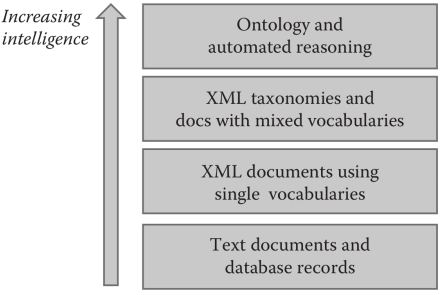
\includegraphics[width=0.7\linewidth]{images/kos-levels}
            \fdireta{9780123859662}
        \end{figure}
        
        Segundo \citeonline{Noy2001}, uma ontologia é especificada pelos seguintes componentes:
        
        \begin{itemize}
        	\item Classes: descrevem os conceitos de um domínio, habilitando a classificação e organização dos indivíduos em um sistema lógico e hierárquico;
            \item Indivíduos: são as instâncias das classes, utilizados para representar elementos específicos, os objetos de interesse do domínio;
            \item Relações: representam as interações entre os conceitos de um domínio e as propriedades presentes nas classes e indivíduos, podendo ter características próprias; 
            \item Axiomas: modelam as regras assumidas como verdadeiras no domínio considerado, sendo possível associar relacionamentos entre indivíduos além de fornecer características descritivas e lógicas para as classes.
        \end{itemize}
        
        A partir dessas definições, existem padrões adotados pela comunidade para implementar os conceitos da Web Semântica. RDF e OWL são alguns dos padrões recomendados pela W3C e que serão apresentados a seguir.
        
	\subsection{\textit{Resource Description Framework} e \textit{Web Ontology Language}}
    
    	RDF é um modelo padrão para intercâmbio de dados para que estes sejam compartilhados e reusados por meio das fronteiras das aplicações, empresas e comunidades. O RDF é usado em diferentes domínios de aplicação como \textit{resource discovery} com o objetivo de aprimorar as capacidades dos motores de busca, catalogação de documentos, descrição de conteúdo e suas relações e descrição de propriedade intelectual. Seu modelo consiste em um conjunto de três tipos de objetos, chamados de tripla RDF. Os componentes são:
        
        \begin{itemize}
        	\item Sujeito: representa os recursos e são identificados por meios de URIs;
            \item Predicado:representa os aspectos, características, atributos ou relações específicas que descrevem o sujeito, onde cada predicado possui um valor específico e relaciona um sujeito a um objeto;
            \item Objeto: um valor de uma propriedade ou um recurso específico que representa uma característica do sujeito.
        \end{itemize}
        
        Com triplas RDF é possível explicitar relações entre dois objetos, mas não é possível fazer modelagens mais expressivas nem mesmo inferências. Para alcançar essas características é necessário que a ontologia seja descrita em OWL.
        
        OWL é uma linguagem recomendada pela W3C para representação e compartilhamento de ontologias na \textit{Web}. Ela foi projetada para aplicações que necessitam processar a informação ao invés de apenas organizá-las em nós \cite{Mcguinness2004}. OWL permite que a semântica seja explicitamente associada ao conteúdo dos dados na \textit{web} e formalmente especificada por meio de ontologias compartilhadas na \textit{internet}.
        
        \begin{figure}[htbp]
        	\centering
            \caption{Diagrama de Venn sobre o relacionamento estre os perfis da linguagem OWL2.}
            \label{fig:owl2-profiles}
            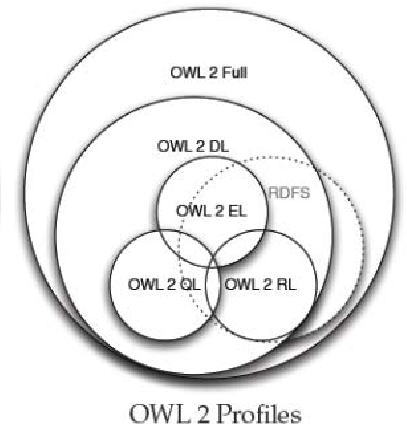
\includegraphics[width=0.7\linewidth]{images/owl2-profiles}
            \fadaptada{Alamri_2012}
        \end{figure}
        
        A versão mais recente desta linguagem é a OWL2 que possui cinco diferentes perfis (sub-linguagens), como pode ser visto na \autoref{fig:owl2-profiles}. Cada um desses perfis permite um nível diferente de expressividade para cada cenário de aplicação. Esses perfis são:
        
        \begin{itemize}
        	\item Full: permite a máxima expressividade e liberdade sintática mas sem garantia computacional;
            \item DL: desenvolvido para aplicações que requerem a máxima expressividade enquanto mantém a decidibilidade (computações terminam em tempo finito) e computabilidade (conclusões são garantidas de serem computáveis). Nesse perfil existem limitações sobre os recursos da linguagem para garantir as duas características citadas anteriormente;
            \item EL: baseado em lógica descritiva, é útil para aplicações que contém um grande número de propriedades e/ou classes;
            \item QL: permite o processo de raciocínio, do inglês \textit{reasoning}, eficiente para grandes quantidades de dados estruturados em ontologias relativamente simples;
            \item RL: direcionado para aplicações que exigem \textit{reasoning} escalável em troca de restrições na expressividade. Favorece a implementação utilizando tecnologias baseadas em regras.
        \end{itemize}

\section{Considerações Finais}

Neste capítulo, procurou-se realizar o embasamento necessário para que se possar ter um entendimento claro do tema desta pesquisa e ainda apresentar uma visão geral das técnicas que serão utilizadas para resolução do problema de pesquisa. A maiorias das referências apresentadas têm, como seu foco principal, o cenário brasileiro, que é onde se deseja implementar a proposta.


\chapter{Trabalhos Relacionados}
\label{chapter:trabalhos-relacionados}
Com o objetivo de relacionar trabalhos já desenvolvidos sobre o tema desta pesquisa para que forneçam ideias e exemplos de abordagem para solucionar o problema apresentado, realizou-se uma pesquisa bibliográfica sobre SADs que utilizaram ontologias de domínio dos especialistas para representar o conhecimento e sistemas similares ao SustenAgro e ao protótipo proposto. A seguir são caracterizados tais trabalhos, evidenciando as suas similaridades e diferenças com esta pesquisa.

% Neste capítulo, em cada subseção são apresentados trabalhos que relacionam-se com este, explicitando em cada um onde se diferenciam e onde se assemelham com a proposta desta monografia.
% * <dilvan@gmail.com> 2018-08-03T19:31:48.791Z:
% 
% porque esses trabalhos relacionados? foram os unicos encontrado? sao exemplos representativos do que existe ? voce fez uma pesquisa bibliografica?
% 
% ^.

Lorem ipsum dolor sit amet, consectetur adipiscing elit. Aenean ut consequat libero. Fusce suscipit nisi quis enim mattis, facilisis venenatis dolor posuere. Suspendisse auctor turpis in ante fermentum volutpat. Suspendisse in sollicitudin felis. Quisque gravida nisl metus. Nam eget iaculis justo. Nunc nec vulputate nisl. Pellentesque semper magna vel nisi pellentesque, sed accumsan purus aliquet. Sed viverra ante turpis, quis tincidunt nulla lobortis sit amet. Sed vitae urna quis elit condimentum venenatis et vitae quam. Donec id risus felis. Ut ac posuere velit. Lorem ipsum dolor sit amet, consectetur adipiscing elit. Vestibulum ante ipsum primis in faucibus orci luctus et ultrices posuere cubilia Curae; Sed in convallis leo.

Cras enim urna, consequat consectetur mi a, laoreet elementum neque. Praesent at eleifend velit, vitae laoreet purus. Vestibulum pulvinar nec sem pretium suscipit. Duis quam erat, consectetur et ipsum eget, ultrices egestas ante. Donec ut quam eu sem malesuada dapibus. Sed ullamcorper metus ac dolor dictum, a facilisis orci bibendum. Proin malesuada, nunc in elementum maximus, lacus dui ullamcorper nisl, at iaculis risus odio at urna. Suspendisse pulvinar lectus at augue tristique, id mattis leo ornare. Vestibulum ante ipsum primis in faucibus orci luctus et ultrices posuere cubilia Curae;

Class aptent taciti sociosqu ad litora torquent per conubia nostra, per inceptos himenaeos. Donec lobortis rhoncus justo, ut hendrerit nisl molestie vitae. Quisque neque est, iaculis eget accumsan ut, finibus eget massa. Class aptent taciti sociosqu ad litora torquent per conubia nostra, per inceptos himenaeos. Duis id mi velit. Vivamus laoreet vitae leo quis maximus. Etiam sit amet ex dolor. Curabitur ac tincidunt neque, ac auctor quam. Nam ullamcorper enim sit amet lacus pretium vestibulum.

Nunc in aliquet massa. Vivamus laoreet scelerisque neque, at porta elit placerat id. Aliquam a nibh ex. Nam quis convallis felis, sit amet sagittis ex. Aliquam pellentesque enim ut justo ultricies viverra. Mauris justo enim, accumsan vitae aliquet non, ultrices eget nibh. Nam ut tincidunt felis. Donec ultricies feugiat mi, sit amet efficitur velit commodo vel. Aliquam erat volutpat.

Aliquam erat volutpat. Duis convallis libero a pulvinar posuere. Vivamus blandit a ante quis lobortis. Quisque consectetur ullamcorper tempus. Maecenas eu ornare leo, sit amet varius felis. Nullam mi urna, lobortis eu magna sed, finibus sodales dui. Nulla viverra gravida felis, quis tempus enim suscipit in. Quisque nisi sem, imperdiet vitae nisi ac, feugiat blandit lectus. In hac habitasse platea dictumst. Maecenas ut massa eget libero iaculis fringilla id id nisi. Fusce pretium nisi nec efficitur ornare. Phasellus lacinia cursus lectus non fermentum. Nam posuere justo et leo venenatis eleifend. Nam ut diam eu felis posuere aliquam et a lorem. Nullam luctus bibendum nibh, quis accumsan nibh pharetra nec.

Pellentesque in est turpis. Vestibulum vel lorem ut mauris tempor accumsan. Suspendisse condimentum, arcu sit amet mollis finibus, est augue mollis risus, in sagittis velit velit id eros. Integer laoreet ante ut odio porttitor, a posuere enim fermentum. Mauris sagittis massa id egestas feugiat. Donec quis libero mauris. Curabitur a scelerisque ipsum. Aliquam erat volutpat. Morbi ut risus tincidunt, lacinia eros et, pharetra augue. Integer porta in nunc sollicitudin placerat. Morbi maximus, dolor a luctus sagittis, dui velit bibendum lacus, at lacinia nibh nibh a nulla. Cras et euismod arcu. Nullam tellus lorem, varius quis tellus eget, fringilla eleifend mi. Aliquam nec nunc et lorem congue tincidunt rutrum at ligula. Nulla blandit vitae leo sit amet ultricies.

Suspendisse at leo eget nisi venenatis scelerisque. Phasellus vulputate sollicitudin enim, sed ornare massa vulputate quis. Ut et diam mollis, vulputate odio et, fermentum erat. Aliquam maximus ut neque sit amet vehicula. Ut sed luctus nunc. Donec augue nisi, accumsan varius facilisis ac, venenatis sit amet lorem. Aenean eu augue felis. Sed vitae consequat turpis. Morbi non lorem non lorem sagittis ullamcorper. Nulla sodales quam non turpis interdum, in tempus arcu laoreet. Donec nec arcu eget quam rutrum ullamcorper sed tempor libero. Mauris rhoncus varius libero, id placerat nunc dictum vitae. Aenean maximus, nisi id feugiat porta, sem velit lobortis est, mollis malesuada nulla nisl non tortor. Nullam nisi eros, ullamcorper mattis luctus eu, eleifend auctor nulla.

Morbi non tempus justo. Fusce cursus orci tellus, in varius sem mollis eu. In hac habitasse platea dictumst. Integer fermentum interdum diam vitae vehicula. Sed et porta leo. Duis quis ante posuere, lacinia sem eget, varius enim. In pellentesque diam vel tellus faucibus, eu tincidunt justo posuere. Nulla ac felis sed eros pretium consectetur id in odio. Ut ligula velit, dictum ultricies scelerisque nec, rhoncus sagittis ante. Donec eget augue id mi lacinia ornare. Nunc consequat consectetur cursus.

Sed interdum congue purus at tincidunt. Vestibulum ante ipsum primis in faucibus orci luctus et ultrices posuere cubilia Curae; Fusce convallis accumsan sem, nec facilisis nibh sodales in. Sed eget tortor nec arcu commodo vestibulum. Vivamus tempor ac lacus et porttitor. Nam enim orci, posuere id sem quis, molestie maximus ligula. Etiam fringilla ante neque, sit amet feugiat lectus finibus quis. Interdum et malesuada fames ac ante ipsum primis in faucibus. Mauris in cursus est. Donec quis sollicitudin magna.

Curabitur faucibus nulla at massa semper accumsan. Proin consequat accumsan ornare. Nam pellentesque convallis viverra. In aliquam ullamcorper leo vel luctus. Praesent sit amet viverra elit. Mauris aliquam felis at metus dictum pharetra. Donec porttitor convallis libero, in posuere urna. Mauris malesuada ornare est. Curabitur quis metus ut urna convallis sagittis. Aenean ac tristique ipsum, et efficitur odio. Morbi eros elit, consectetur a massa et, tincidunt hendrerit nisi. In euismod lorem orci, ut scelerisque odio luctus ut. Pellentesque est sapien, commodo at diam molestie, rutrum molestie augue. Proin luctus, ipsum in tincidunt venenatis, lectus nibh ullamcorper massa, id suscipit ex est vel sem. Nulla id velit a massa convallis ultricies non vel orci.

Mauris libero lectus, ullamcorper blandit mi sed, consequat finibus libero. Etiam quam ex, maximus vel tristique ut, dictum eget massa. Sed vel aliquet urna, vel fermentum ligula. Aliquam vulputate sagittis varius. Phasellus aliquam metus ac turpis ultricies hendrerit. Maecenas rutrum tincidunt eros ut auctor. Nullam mollis massa non feugiat facilisis. Nunc felis ipsum, dapibus et quam nec, scelerisque accumsan nisi. Nulla est sapien, tempus eget congue eget, lobortis maximus dui. Nam vehicula eros eu leo facilisis, sit amet congue ante scelerisque. Maecenas vel velit ultrices, venenatis tellus non, pellentesque lacus. Praesent dictum urna quam, quis interdum nisl viverra dignissim. Donec odio justo, condimentum sit amet tristique id, pretium eu enim. Aliquam aliquet imperdiet quam, a semper leo lobortis ac.

Nullam volutpat elementum egestas. Nulla aliquet mattis consectetur. Ut volutpat non metus a iaculis. Mauris tincidunt ante orci, commodo cursus turpis pharetra eu. In consequat lorem sit amet mauris volutpat, ac cursus erat interdum. Praesent sit amet ullamcorper urna. Etiam rhoncus justo malesuada, viverra turpis non, efficitur velit. Maecenas a rutrum turpis. Nullam porta, erat eget lobortis fermentum, risus orci sagittis massa, sed congue metus enim sit amet nisi. Mauris gravida lectus nisi, nec molestie enim hendrerit non. Praesent tincidunt metus nec mauris eleifend pharetra. Aenean viverra justo ac urna molestie, a tincidunt nisi blandit. Morbi id odio non arcu varius vehicula.

Interdum et malesuada fames ac ante ipsum primis in faucibus. Fusce faucibus ante fringilla ultricies consequat. Quisque porta justo nec commodo euismod. Vestibulum aliquam leo enim, ut mollis sapien dapibus eget. Integer a justo vel erat consequat scelerisque semper quis eros. Curabitur a congue ante. Suspendisse tristique, urna sit amet sagittis tincidunt, lectus massa laoreet massa, eu congue nibh tortor et odio. Aenean felis libero, porta interdum dui at, consectetur vehicula dolor. Ut porttitor viverra mauris, ut suscipit diam semper id. Nunc ac vulputate sapien. Nulla lacinia pulvinar sodales. Nulla eget diam vel enim tristique interdum eget a est. Praesent sit amet nibh mauris. Praesent ac interdum neque. Ut non nisl tincidunt nunc pulvinar consequat vel sed purus. Aliquam posuere interdum fringilla.

\section{Considerações Finais}
% * <dilvan@gmail.com> 2018-08-03T19:45:00.783Z:
% 
% ficou fraco. os 3 exemplos sao do grupo da katia. so eles trabalham com sads? porque nao ha exemplos de outros grupos? ninguem faz nada remotamente relacionado? como voce chegou a essa conclusao?
% 
% ^.
	Neste capítulo procurou-se apresentar trabalhos relacionados que utilizam tecnologias ou técnicas iguais ou similares à proposta apresentada nesta monografia, com o objetivo de evidenciar a relevância da metodologia adotada por este trabalho no contexto científico. A partir dos trabalhos apresentados é possível destacar o papel das ontologias no desenvolvimento de SADs em diferentes domínios e a ausência de mecanismos que permitam os especialistas do domínio alterar o comportamento destes sistemas sem que se faça necessário um contato com desenvolvedores de \textit{software}. A proposta é caracterizada com mais detalhes no próximo capítulo.

\chapter{Proposta}
\label{chapter:proposta}
Este capítulo apresenta o problema identificado, a proposta de resolução para este problema, o planejamento de ações para alcançar a solução e os resultados que são esperados ao fim da pesquisa.



\section{Metodologia}
\label{sec:methodology}

 Para a resolução do problema apresentado, é proposto a criação de uma ontologia que contemple  as propriedades necessárias de pacientes a serem atendidos em uma especialidade médica e um protótipo que utilize estes itens e gerencie uma fila de espera de acordo com critérios preestabelecidos por médicos.

    Com o intuito de validar a proposta, será desenvolvido um estudo de caso com o Hospital das Clínicas da Faculdade de Medicina de Marília (FAMEMA), onde se espera implantar a ontologia e o protótipo. Posteriormente solicitar a médicos que avaliem o gerenciamento realizado pelo protótipo, e informem qual a concordância com a fila gerenciada de acordo com a quantidade de pacientes que julgarem estar corretamente posicionados, e para efeito de comparação também informarem qual a concordância da fila de atendimento gerenciada antes da implantação do protótipo, permitindo assim analisar se a proposta de fato pode gerenciar uma fila de espera de forma mais eficaz na visão dos especialistas (médicos).
	
	O intuito não é discutir quais deverão ser critérios utilizados pelos médicos para avaliar se um paciente X tem prioridade em relação ao paciente Y, mas sim possibilitar que a partir de critérios previamente estabelecidos, o computador possa fazer esta triagem de forma eficaz, sem a necessidade de alocação de um médico para uma avaliação caso a caso, e nem que funcionários administrativos façam esse ordenamento, almejando um ordenamento mais próximo ao que os médicos aconselham, sendo mais justa e transparente uma fila de atendimento. 
	
	O método para se chegar ao objetivo desta pesquisa é utilizar recursos da web semântica, como a ontologia para que se possa representar itens de pacientes que poderão ser utilizados para gerenciar uma fila de espera.

    \section{Cronograma}

	Considerando um tempo de 25 meses para o desenvolvimento da pesquisa proposta e a numeração das tarefas apresentadas na \autoref{sec:methodology}, o cronograma das atividades se apresenta na Tabela 1 %\autoref{tab:cronogram}.
	
	  \begin{enumerate}
    	\item Conclusão da validação do exame de proficiência em língua estrangeira;
        \item Integralização dos créditos obrigatórios;
        \item Mapeamento da literatura;
        \item Elaboração e apresentação dos artefatos relacionados ao exame de qualificação;
         \item Desenvolvimento da ontologia OWL que represente indicadores para classificação de prioridades para o atendimento de uma especialidade médica;
        \item Desenvolvimento e testes de um protótipo que utilize a ontologia desenvolvida e gerencie uma fila de espera utilizando critérios definidos;
        \item Elaboração e submissão de artigos;
        \item Elaboração e apresentação dos artefatos relacionados a defesa;
    \end{enumerate}
    
    \begin{table}[htbp]
    	\centering
        \caption{Cronograma das atividades da pesquisa.}
        \label{tab:cronogram}
        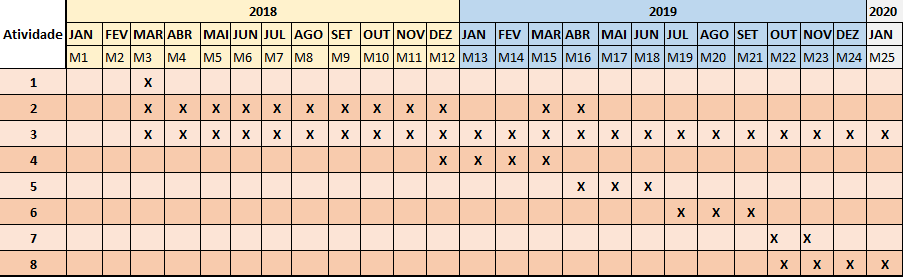
\includegraphics[width=1\linewidth]{images/cronogram}
        \fautor
    \end{table}
    
    \pagebreak
    
   \section{ Resultados Esperados}

	Ao final desta pesquisa espera-se as seguintes contribuições:
	
	\begin{itemize}
		\item Uma ontologia OWL que represente indicadores para classificação de prioridades para o atendimento de uma especialidade médica;
        \item  Um protótipo que gerencie filas de espera computacionalmente e se mostre  mais eficaz que o gerenciamento atual do HC FAMEMA;
        \item Estudo de caso mostre que o modelo proposto pode auxiliar na gestão de filas do Sistema Único de Saúde e obter benefícios se comparadas as outras formas de gerenciamento;
	\end{itemize}



% ---
% Finaliza a parte no bookmark do PDF, para que se inicie o bookmark na raiz
% ---
\bookmarksetup{startatroot}% 
% ---

% ----------------------------------------------------------
% ELEMENTOS PÓS-TEXTUAIS
% ----------------------------------------------------------
\postextual

% ----------------------------------------------------------
% Referências bibliográficas
% ----------------------------------------------------------
\bibliography{references}

\end{document}